\pdfminorversion=4
\pdfobjcompresslevel=1

\documentclass{beamer}
%\usetheme{Warsaw}
\usetheme{MAUA}
\setlength{\leftmargini}{20pt}

\usepackage[utf8]{inputenc}
\usepackage[T1]{fontenc}
\usepackage{minted}
\usepackage[brazil,brazilian]{babel}

\usepackage{tikz-timing}[2009/05/15]
\def\degr{${}^\circ$}

\usepackage{mdframed}
\definecolor{pearl}{rgb}{0.94, 0.92, 0.84}

\usepackage{graphicx}
\graphicspath{./Figs/}

\usepackage{todonotes}

\title{Processamento de Sinais}
\subtitle{HIL}
\author{Rafael Corsi Ferrão}
\date{\today}
\institute{\url{rafael.corsi@maua.br}}

\AtBeginSection[]
  {
     \begin{frame}<beamer>
     \frametitle{Conteúdo}
     \tableofcontents[currentsection]
     \end{frame}
}  

\begin{document}

\begin{frame}[plain,t]
	\titlepage
\end{frame}

\begin{frame}
	\frametitle{Conteúdo}
		\tableofcontents
\end{frame}

\section{HIL}

\subsection{Introdução}

\begin{frame}{Filtros Digitais}

Filtros são utilizados por basicamente dois motivos:

\begin{itemize}
\item Separar um sinal de outro
\item Reparar um sinal que sofreu distorção
\end{itemize}

Existem dois tipos de filtros digitais:

\begin{itemize}
	\item FIR: Finite Impulse Response
	\item IIR: Infinite Impulse Response
\end{itemize}

\end{frame}

\section{IIR}
\begin{frame}{IIR}

	\[
		H(z) = \frac{B(z)}{Y(z)} = \frac{b_0 + b_1 z^{-1} + \ldots + b_m z^{-m}}{1 + a_1 z^{-1} + \ldots + a_m z^{-m}}
	\]


	\begin{itemize}
		\item Filtro recursivo
		\item Analogia com filtros analógicos
		\item Possui pólos e zeros
	\end{itemize}
\end{frame}

\begin{frame}{IIR}{implementação}
	\begin{center}
	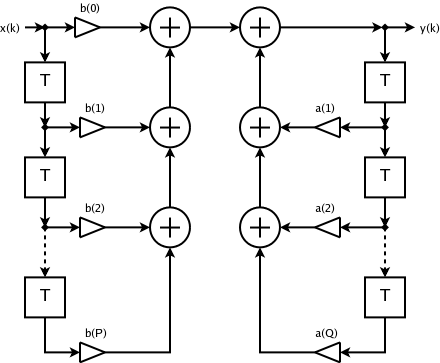
\includegraphics[width=0.7\linewidth]{IIR-filter}
	\end{center}
\end{frame}

\section{FIR}

\begin{frame}{FIR}

	\[
		H(z) = B(z) = \sum_{k=0}^{M} b_z z^{-k}
	\]

	\begin{itemize}
		\item Média móvel
		\item Convolução
		\item Sempre estáveis
		\item Fase linear 
	\end{itemize}
\end{frame}

\begin{frame}{IIR}{implementação}
	\begin{center}
	
\includegraphics[width=1\linewidth]{fir-filter}
	\end{center}
	
	Basta escolher os pesos (b)

\end{frame}

\begin{frame}{Janelas}

	Como escolher os pesos (b) ?	
	\pause

	\begin{center}
	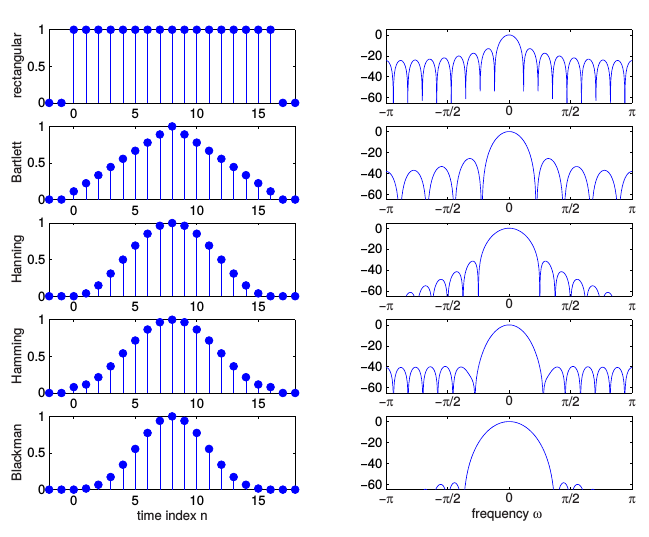
\includegraphics[width=0.8\linewidth]{fir_janelas}
	\end{center}
\end{frame}

\section{Matlab}

\begin{frame}{Projetando o filtro}
	
	Para projetarmos o filtro, iremos utilizar o tool box: \textit{Filter Design \& Analysis} do Matlab (Versão >= 2012), 
	
\begin{center}
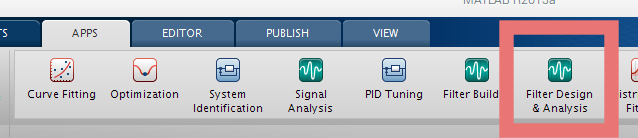
\includegraphics[width=0.7\linewidth]{matlab1}
\end{center}

\end{frame}

\begin{frame}{Filtro}{Projeto}
\begin{center}
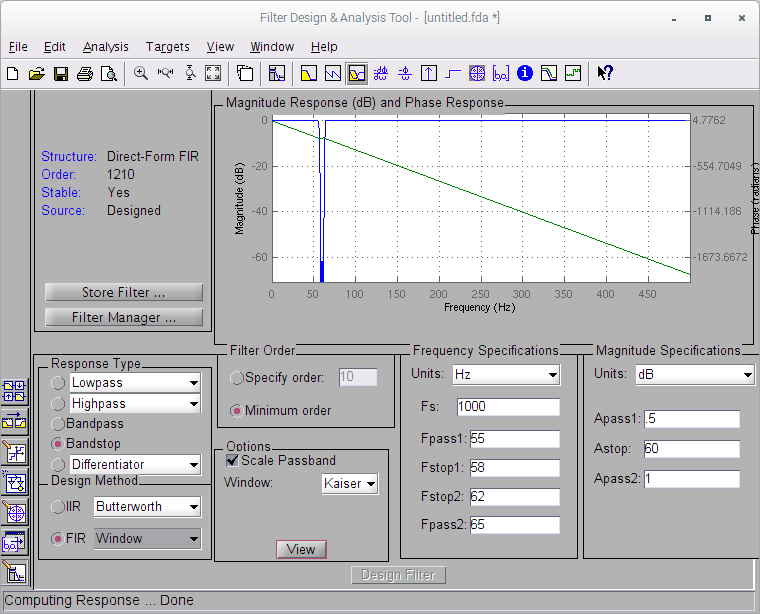
\includegraphics[width=1\linewidth]{matlab2}
\end{center}
\end{frame}

\begin{frame}{Filtro}{Simulink}
\begin{center}
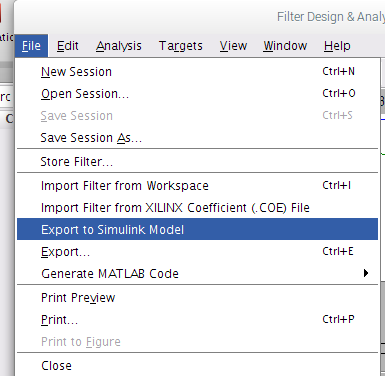
\includegraphics[width=0.5\linewidth]{matlab3}
\end{center}
\end{frame}


% % % % % % % % % % % % % % %
\end{document}
% % % % % % % % % % % % % % %

